\documentclass[10pt,twocolumn,letterpaper]{article}

\usepackage{cvpr}
\usepackage{times}
\usepackage{epsfig}
\usepackage{graphicx}
\usepackage{amsmath}
\usepackage{amssymb}

% Include other packages here, before hyperref.

% If you comment hyperref and then uncomment it, you should delete
% egpaper.aux before re-running latex.  (Or just hit 'q' on the first latex
% run, let it finish, and you should be clear).
\usepackage[pagebackref=true,breaklinks=true,letterpaper=true,colorlinks,bookmarks=false]{hyperref}

\cvprfinalcopy % *** Uncomment this line for the final submission

\def\cvprPaperID{****} % *** Enter the CVPR Paper ID here
\def\httilde{\mbox{\tt\raisebox{-.5ex}{\symbol{126}}}}

% Define a new environment for text boxes
\newenvironment{itextbox}[1]
{\par\begin{center}
\begin{tabular}{|p{0.45\textwidth}|}
\hline
\textbf{#1} \\
\hline
\itshape\ignorespaces
}
{\\\hline
\end{tabular}
\end{center}\par}

% Pages are numbered in submission mode, and unnumbered in camera-ready
\ifcvprfinal\pagestyle{empty}\fi
\begin{document}

%%%%%%%%% TITLE
\title{Project Report : CS 7643 (Temporal title)}

\author{Rilsky Viktor\\
Georgia Institute of Technology\\
{\tt\small vrilsky3@gatech.edu}
% For a paper whose authors are all at the same institution,
% omit the following lines up until the closing ``}''.
% Additional authors and addresses can be added with ``\and'',
% just like the second author.
% To save space, use either the email address or home page, not both
\and
Pandurangan Suriyanarayna G\\
Georgia Institute of Technology\\
{\tt\small ganesan.pandurangan@gatech.edu}
\and
Lu Shuyan\\
Georgia Institute of Technology\\
{\tt\small slu336@gatech.edu}
\and
Hoyeob Kim\\
Georgia Institute of Technology\\
{\tt\small hkim3217@gatech.edu}
}

\maketitle
%\thispagestyle{empty}

%%%%%%%%% ABSTRACT
%\begin{abstract}
%   The ABSTRACT To be written
%\end{abstract}

%%%%%%%%% BODY TEXT
\section{Introduction/Background/Motivation}
%subsection{Motivation}
In recent years, LLM(Large Language Models) applications drew people’s attention as they have demonstrated astonishing conversational interactive experiences. Questions from the public soon follow on the capabilities of LLM, and the extent of the technology’s potential. Interestingly, many tasks that LLMs struggle with point to the same challenge, which is the limited context window. As existing language models are generally implemented with transformers, they require memory and computation resources that increase quadratically in sequence length which puts a limit on the context length. In this article, we look into this limited context window problem or similarly, how to learn from examples more efficiently, and experiment with both fine-tuning and in-context learning methods that aim at alleviating it, increasing both in-domain and out-of-domain accuracy on RTE dataset.

There are multiple investigated approaches to improve the context window limit. The first approach involves architectural changes that develops and trains models with longer context length from scratch. The other type, while keeping the architecture and pre-trained model intact, leverages the idea of adaptation and adapts the LLMs to tasks that are under a unique context. The classic adaptation methodologies of fine-tuning and in-context learning falls under this latter category. 

In ICL, we adapt a model to a task by conditioning it on a sequence of demonstrations. A demonstration typically refers to an input x accompanied by its ground-truth label y, both of which often are converted to a specific pattern format. ICL thus feeds the model a sequence of such demonstrations, followed by the test input. The language model is then expected to predict the label of this final data point.

Pattern-based fine-tuning (PBFT) is a recently proposed FT approach that uses the pretrained language modeling head instead of a randomly initialized classifier. Compared to vanilla FT, we have to specify an input pattern (to cast the task as a language modeling problem) and define a verbalizer (which maps tokens in the pre-trained model’s vocabulary to labels; Schick et al., 2020). For example, a NLI pattern might look as follows: {premise} Question:{hypothesis} Yes or No?,and the verbalizer will use Yes and No as tokens. Given these inputs and targets, model parameters are fine-tuned as usual. This method has been shown to be efficient for few-shot learning despite having no advantage over vanilla FT when the number of examples is large.
Recent work has argued that ICL leads to better out-of-domain performance, when compared to FT (Si et al., 2023; Awadalla et al., 2022). LLMFT paper show that this often does not hold, proving the potential in non ICL context-aware inference. 
There are many real-life and business use cases that could benefit from a long context window. For example, When Google tested its Gemini 1.5 which was released February 2024, they dropped an entire codebase and asked Gemini to write documentation for it. They also showed a 45-minute movie to Gemini and asked questions about the movie. To add on to that, use cases can be reading homeworks from current and all history class sessions to locate possible plagiarisation, to read detailed customer service chat history and chat instructions to tune a customer service chatbot, to monitor the videos online, etc. Theoretically, anything that exceeds the standard context window, which is around 124k tokens for GPT-4 and LLMs alike, compiled PDF files, details instructions, movies or videos longer than 5 minutes (videos are pre-processed into frames and each frame count as 128 tokens roughly) would be challenging for current LLMs. And It will be more challenging if more than one type of data is provided, for example, have LLMs to watch a 2 hour movie and write reviews or press articles about the movie. The actual use cases have no limit.

We use RTE (Recognizing Textual Entailment) dataset in this experimentation. The RTE datasets come from a series of textual entailment challenges. It started with “an inference test suite for evaluating the inferential competence of different NLP systems and semantic theories” called FraCas which is created manually by many linguists and funded by FP3-LRE. Later, Pascal RTE challenges, sharing a similar goal as FraCas, starts this RTE generic evaluation framework that evaluates models for distinct, real-world downstream tasks so datasets were extracted from downstream tasks through a process referred to as recasting (Glickman, 2006). This framework has impacted the community hugely and has been evolving since. The dataset we use is a combined dataset from RTE1, RTE2, RTE3 and RTE5. Examples are constructed from news and wikipedia text. For out-of-domain evaluations, we use the HANS dataset which is an NLI evaluation set that tests specific hypotheses about invalid heuristics that NLI models are likely to learn.

\begin{table*}
   \begin{center}
   \begin{tabular}{|c|p{6cm}|p{6cm}|c|}
   \hline
   Index & Sentence 1 & Sentence 2 & Label \\
   \hline
   0 & No Weapons of Mass Destruction Found in Iraq Yet. & Weapons of Mass Destruction Found in Iraq. &  1 (not entailment)\\
   \hline
   1 & A place of sorrow, after Pope John Paul II died, became a place of celebration, as Roman Catholic faithful gathered in downtown Chicago to mark the installation of new Pope Benedict XVI. & Pope Benedict XVI is the new leader of the Roman Catholic Church. & 0 (entailment) \\
   \hline
   \end{tabular}
   \end{center}
   \caption{Examples from the development sets of RTE. Each example contains 2 sentences and a label indicating whether sentence 2 can be inferred based on sentence 1.}
   \label{tab:contributions}
\end{table*}
%-------------------------------------------------------------------------
%------------------------------------------------------------------------
\section{Approach}
The idea we propose in this project is to apply the context distillation fine-tuning of
the natural language inference (NLI) classification task and compare it to the ICL approach. Given OPT’s fixed context size of 2048 tokens we are limited in the number of examples we can use at inference time, but the number of examples supplied are not limited during fine tuning. That is to say,  theoretically the limited context window problem can be solved by fine-tuning on the context material.

Now the problem becomes how to enable the pre-trained model to learn more efficiently during fine training. We have attempted to execute context distillation fine-tuning in this project and specifically look into the dynamics of KL Divergence Loss which was not discussed in the literature we went through. 

We based our work on the llmft repo \url{https://github.com/uds-lsv/llmft} which was created along with the Few-shot Fine-tuning vs. In-context Learning paper (Marius et al, 2023). Our fork and code of the project is available here: \url{https://github.com/vrilsky3/deep_learning_project}.

\begin{itextbox}{sample prompt when num of ctx examples = 1}
   \\
   Task: Determine the relationship between the following two sentences. Answer 0 for 'entailment', 1 for 'contradiction'.

   Here are examples  to help you:
   Example 1:
   Sentence1: No Weapons of Mass Destruction Found in Iraq Yet.
   Sentence2: Weapons of Mass Destruction Found in Iraq.
   Answer:  1
   
   Now, please answer the following question: 
   Question:
   Sentence1: Mangla was summoned after Madhumita's sister Nidhi Shukla, who was the first witness in the case      
   Sentence2: Shukla is related to Mangla.  \\        
   Answer:
\end{itextbox}

\subparagraph*{Loss Function}

We designed and implemented a new loss function in order to do context distillation learning with Kullback-Leibler (KL) divergence. The previous existing loss method was simply cross-entropy loss with the expected label. In our loss, we ignore the label. We use context examples ($C$) as specified in the previous dataset section to create a prompt that will represent $X\mid C$, a context enriched input. Then, we pass that to $P_0$, which is a frozen model that we use to generate predictions logits. Of course, at inference we will not have this context, but rather we want the model to learn this context. Therefore, for our model ($P_\theta$), we pass only $X$. Instead of cross-entropy loss, we have the KL divergence which measures distance between distributions (we perform softmax before passing them to the KLD component).
The goal here is to learn not just what is the correct label (the most likely token by $P_0$), but also by using all tokens distribution, this can be see as a knowledge distillation scheme with $P_0$ being the teacher, and $P_0$ as the student. There are about 50k tokens, many of them irrelevant and therefore we only use top K of the tokens (and append the sum of the rest, in order to have the predictions sum to 1). \\
The motivation driving this approach is to learn how to do predictions within a context C without being given C as part of your input.
The idea is that $P_0$ is enriched by the context and provides good predictions given the context domain. 
$P_\theta$ of course is oblivious to the context, it is only aware of the input $X$,
and provides predictions that are oblivious to the context. Finally, optimizing for the KL divergence of the context-aware and context-blind predictions would (hopefully) adjust $P_\theta$’s predictions to take into account the context.


\begin{figure}[htbp]
   \centering
   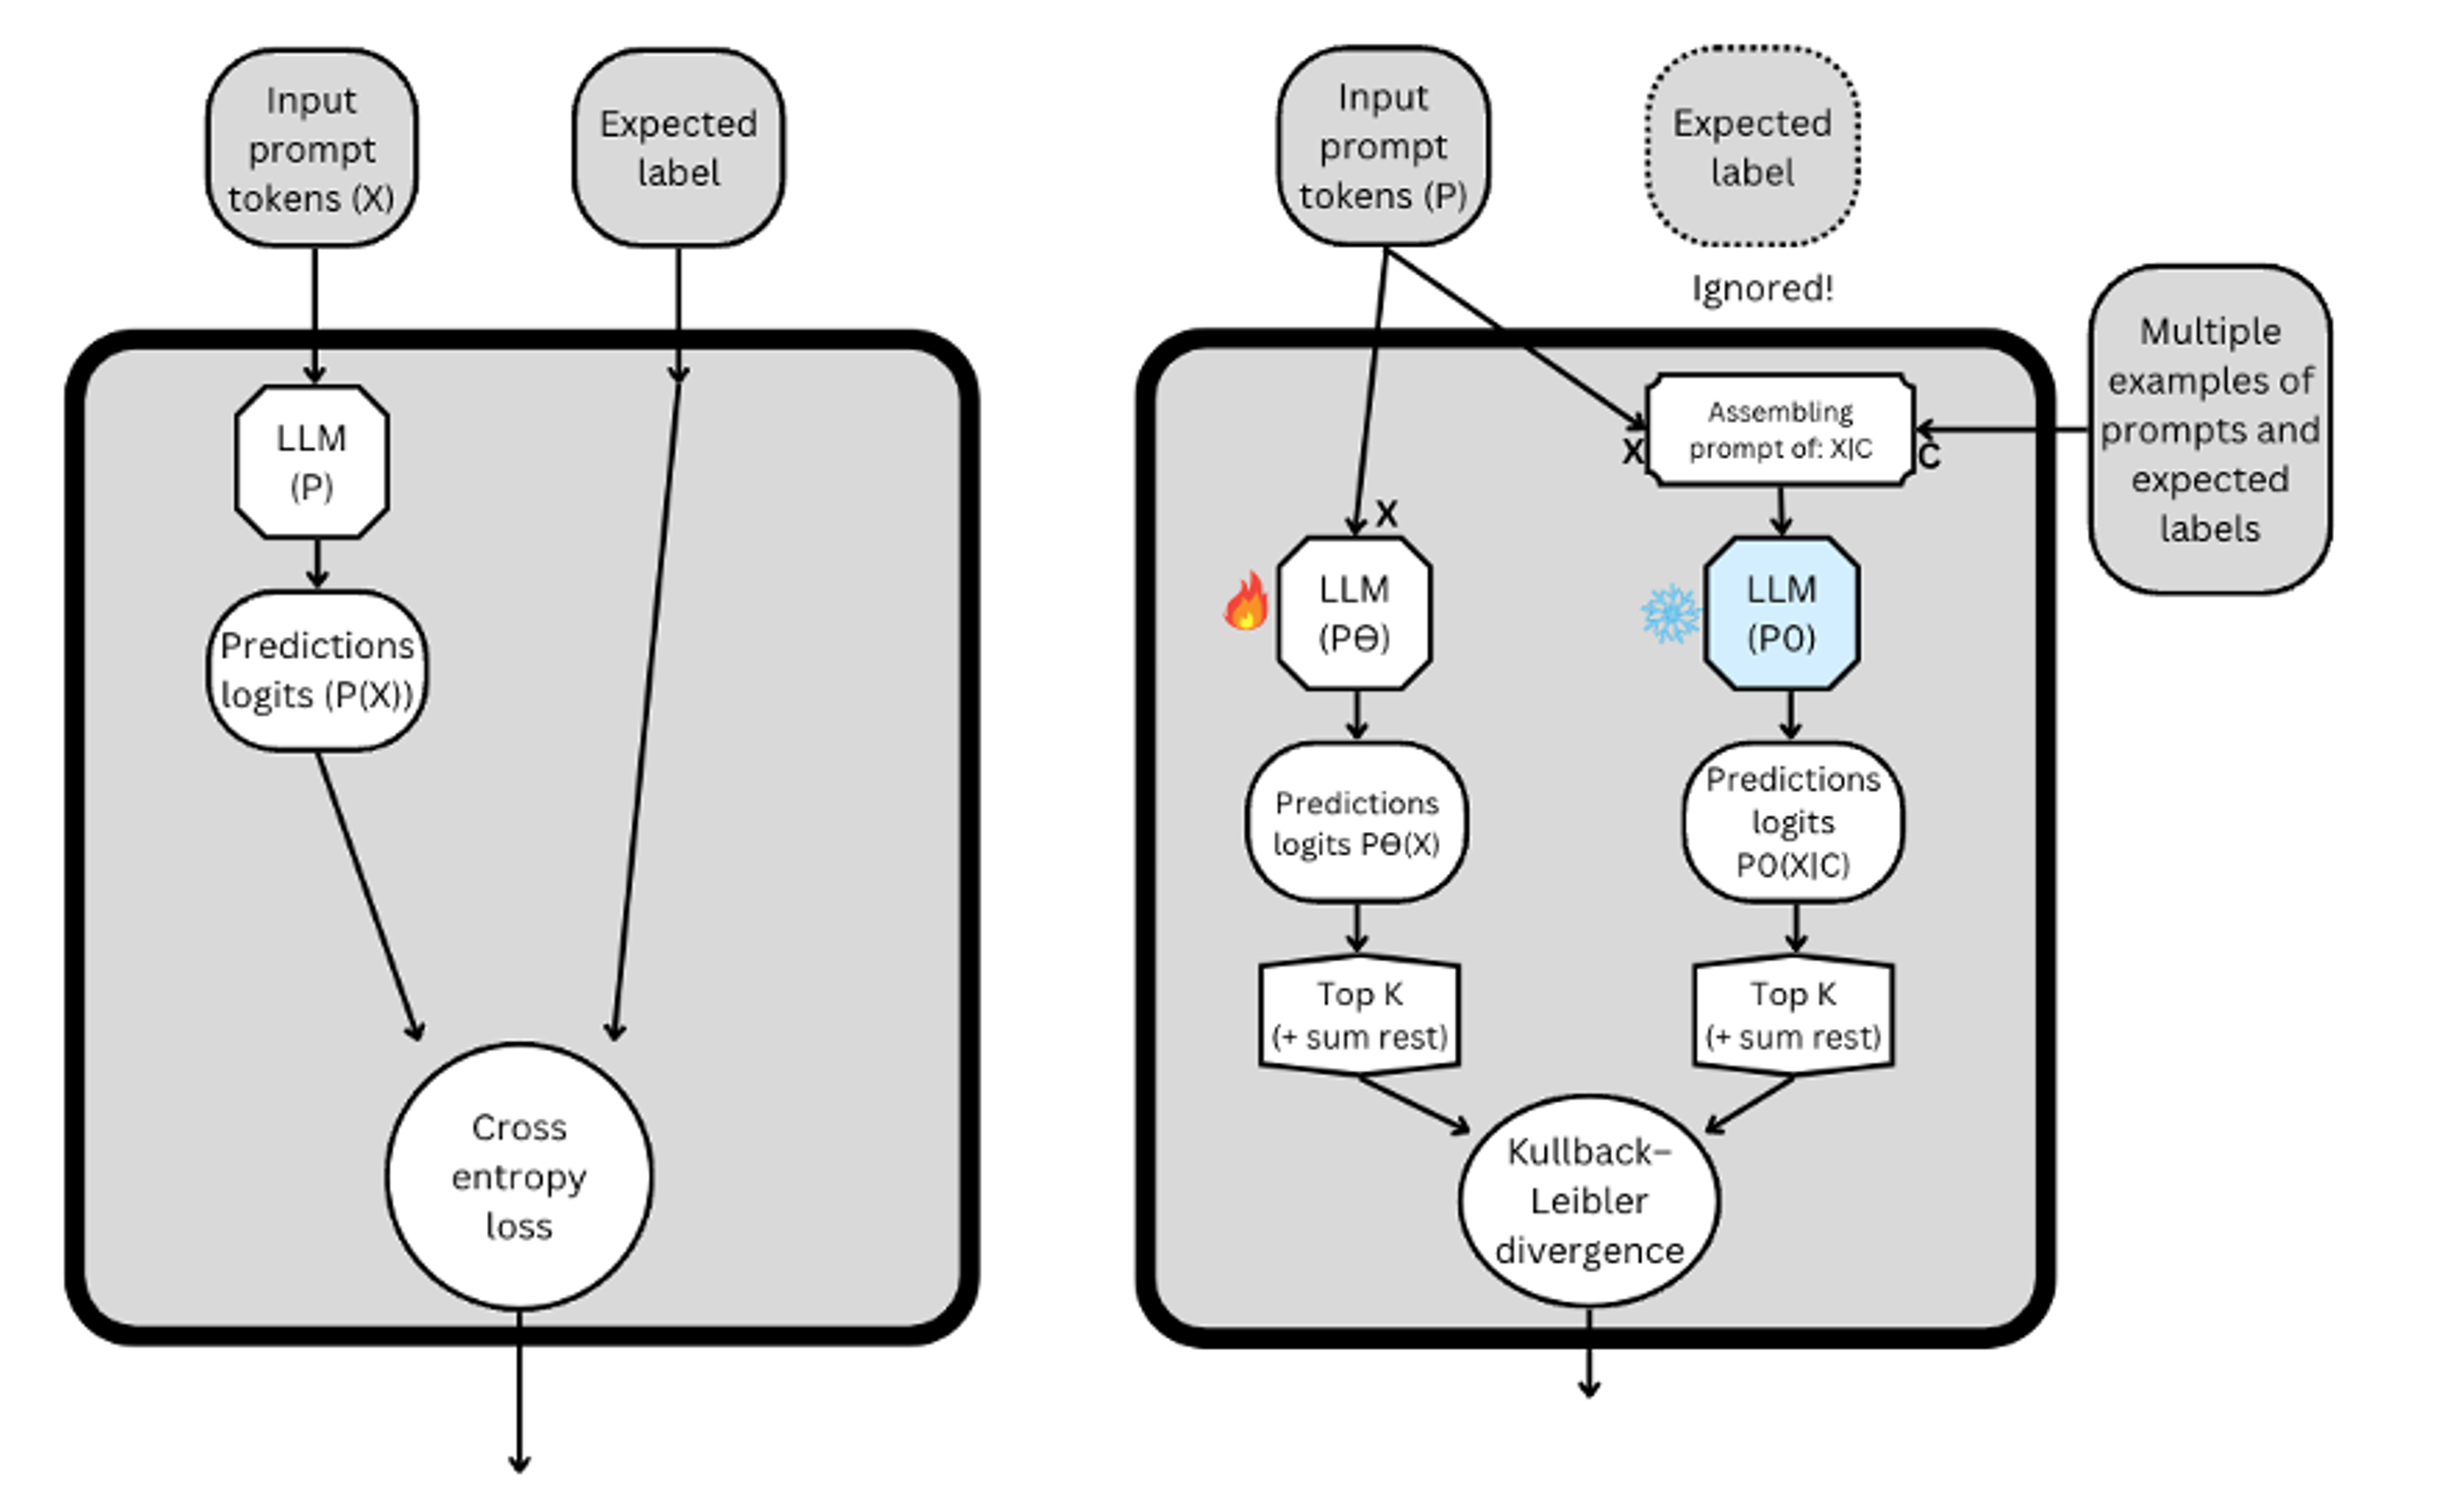
\includegraphics[width=0.50\textwidth]{fig_1_loss_structure_comparison.png}
   \caption{Loss Structure Comparison (left: previous loss, right: our KLD loss).}
   \label{fig:your-label}
\end{figure}



\section{Experiments and Results}


\subsection*{Experimentation goals}
The main hypothesis we rely on is that the new loss method we devised will tune a model that will yield predictions that will improve the accuracy on both in-domain and out-of-domain data. The previous loss method is dependent on the input label, but our new approach only optimizes for the KL divergence of the prediction, which we assume will incorporate the context and thus produce the predictions we want. For this, we need to see that as the loss improves, the accuracy improves as well. 
Furthermore, our method has some parameters we do not know the effect of. Namely the number of context examples that P0 is enriched with, and the number of top K tokens. For this, we compare loss and accuracy with different values.
Lastly, we would like to compare our method to the previous loss fine tuning method. We will compare the accuracy of the resulting models both in-domain and out-of-domain.

\subsection*{Experiments design and setup}
We performed an exploration on the dynamics of optimizing  KL Divergence loss, and compared ICL and FT approaches for task adaptation in NLI by their in-domain and out-of-domain performances. In the following paragraphs, we discuss our experiment setups in detail.

\subparagraph*{Models}
All experiments were run using the same OPT model (Zhang et al., 2022) with 125 million parameters, thus our results can be compared directly without other factors at play. It was also a decision made due to limited computing resources.
We used the 125 million parameter model for both $P_0$ and $P_\theta$. Note that $P_0$ is frozen (we only use it for inference),
 and it may be any other model that uses the same vocabulary. Furthermore, since we train to fit for the predictions of $P_0$,
  it is preferred that $P_0$ be the best model possible, which is often bigger.
   In fact, in the paper that offered this method, they used the largest OPT model (52B).
    Due to compute resource limitation, we used the same model size as $P_\theta$ (125M), which as we will present, ended up degrading our results.
\subparagraph*{ICL setup}
2 number of context examples are provided to ICL. We consider a prediction to be correct when the returned probability of the ground truth’s verbalizer is larger than the other verbalizer token.

\subparagraph*{FT setup}
We perform a few-shot PBFT with the simple pattern shown in the above datasets section where we expect the model to follow up with a 0 or 1 indicating the label for the test case. The number of context examples supplied are tested with different values, either 1 or 2 or 3 examples are provided. The pre-trained model is tuned with KL Divergence loss between the stored log-probabilities and the model-predicted probabilities. The number of log probabilities stored are also tested with different values, either top 5 or 10 or 50 tokens are preserved. LoRA is used as the PEFT technique to speed up the training process.
\linebreak

Only in a late stage of the project, we realized that our GPU memory resources are not able to load big models. As discussed, our entire method heavily relies on $P_0$ to both incorporate the context and provide useful logits to learn from.
We planned to have $P_\theta$ a smaller model, but we absolutely needed $P_0$ to be the biggest model possible, as the context enriched prompt $X \mid P$ is long and much more complicated compared to the single question prompt X that $P_\theta$ is being fed. We still ran the experiments to see what kind of behavior we would see but we anticipated that the accuracy will be low as we are fitting for bad $P_0$ prediction (garbage in - garbage out). 


\subsection*{Results}
We present the results from experimenting the dynamics of KL divergence loss in figure [2] and figure [3], and the in-domain and out-of-domain model performance in Figure [4], comparing both ICL and FT methods.

\subparagraph*{How much OOD data is needed?}
Before experiments, we expect to see the performance getting better when a larger number of context examples are provided. The experiment actually shows that the number of context examples provided relates to the performance at the initial epochs, the difference between the initial performance starts to diminish when the fine tuning process goes further. This proves that our experiments do bring $P_\theta(X)$ close to $P_0(X|C)$.

\subparagraph*{How many tokens are needed in KL divergence loss?}
Before experiments, we expect to see similar performance between the number of tokens as the probabilities of tokens is a skewed distribution where the top couple tokens account for the majority of possiblities. The experiment does confirm our expectations with some caveats covered in the next couple paragraphs.

\begin{figure}[htbp]
   \centering
   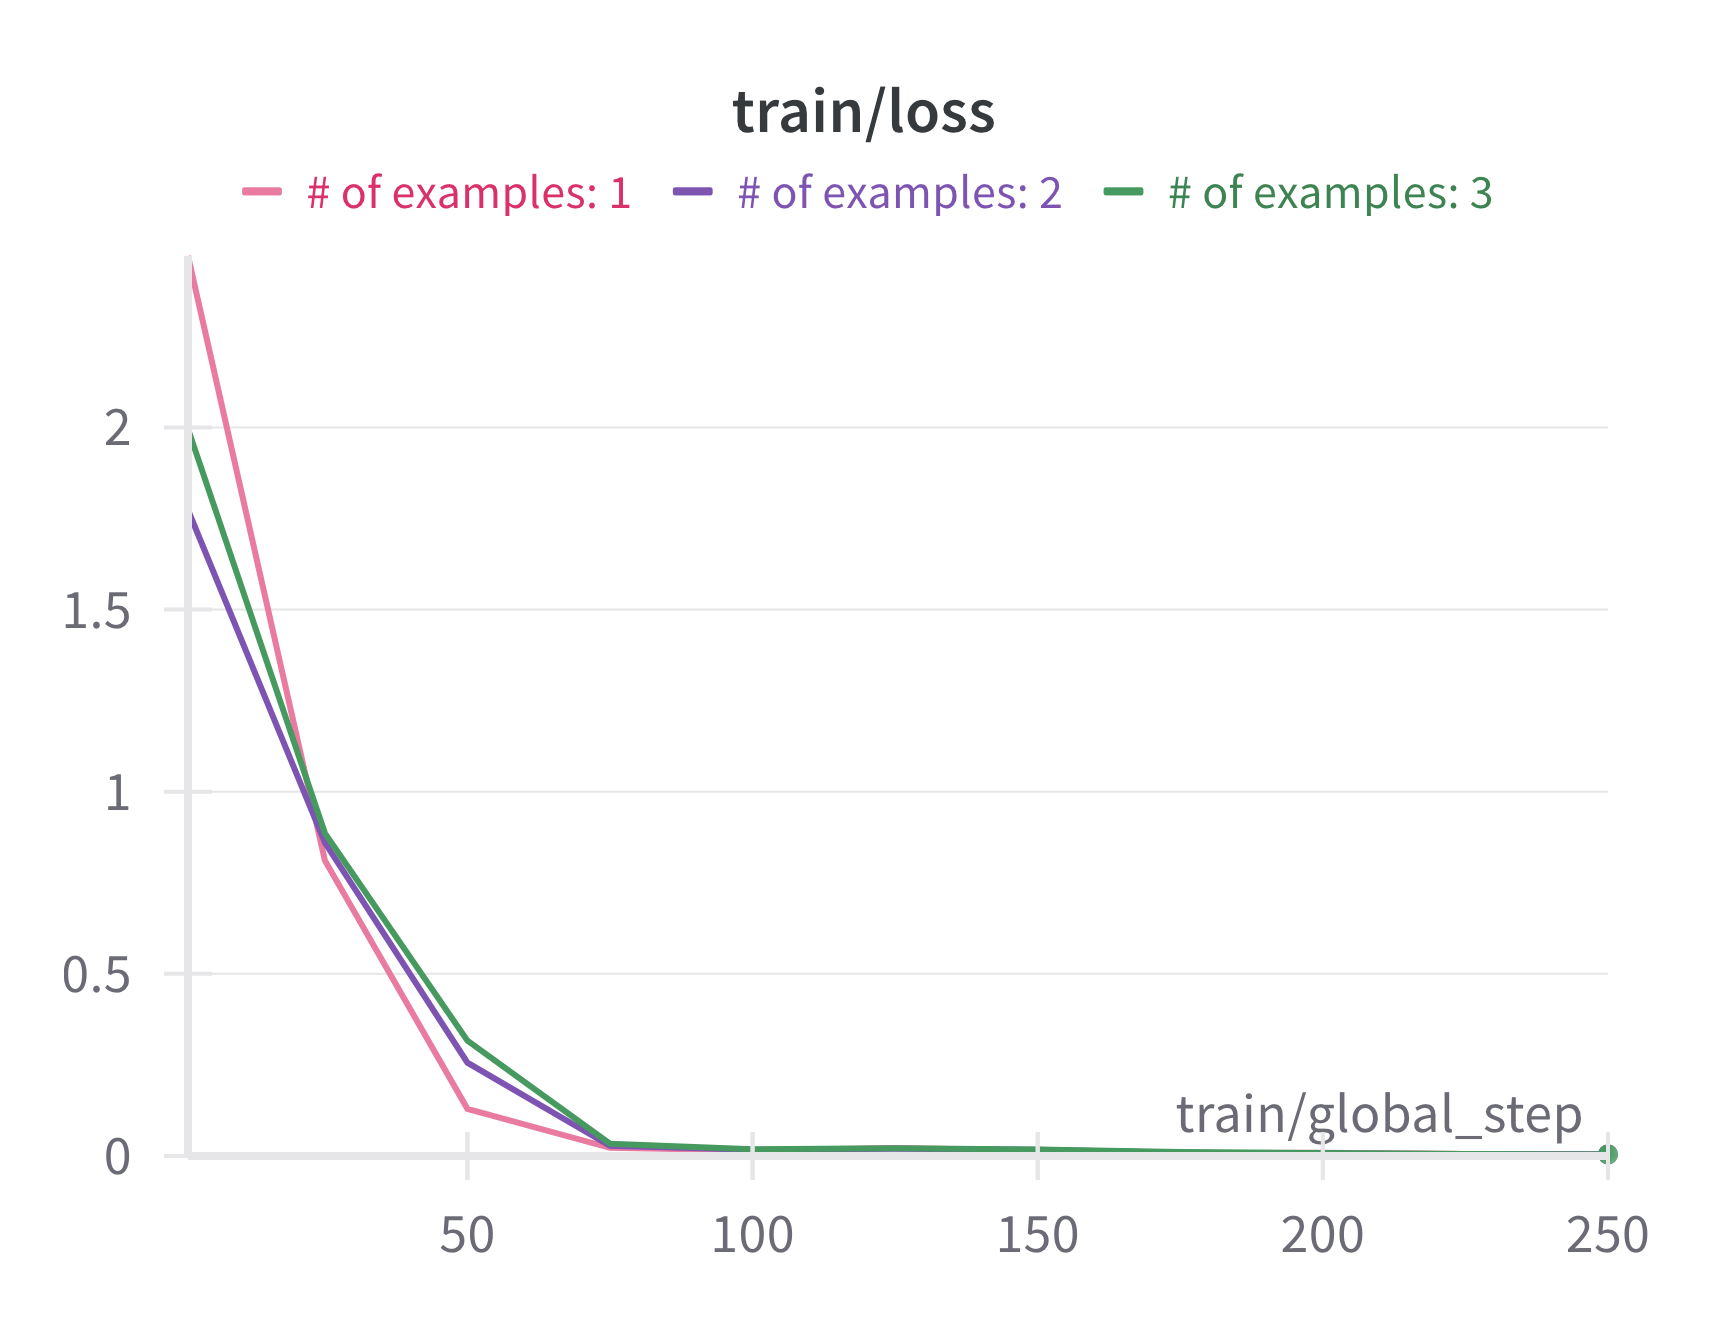
\includegraphics[width=0.50\textwidth]{Fig1_comparing number of context examples.png}
   \caption{PBFT when different number of context examples provided}
   \label{fig:your-label}
\end{figure}




\begin{figure}[htbp]
   \centering
   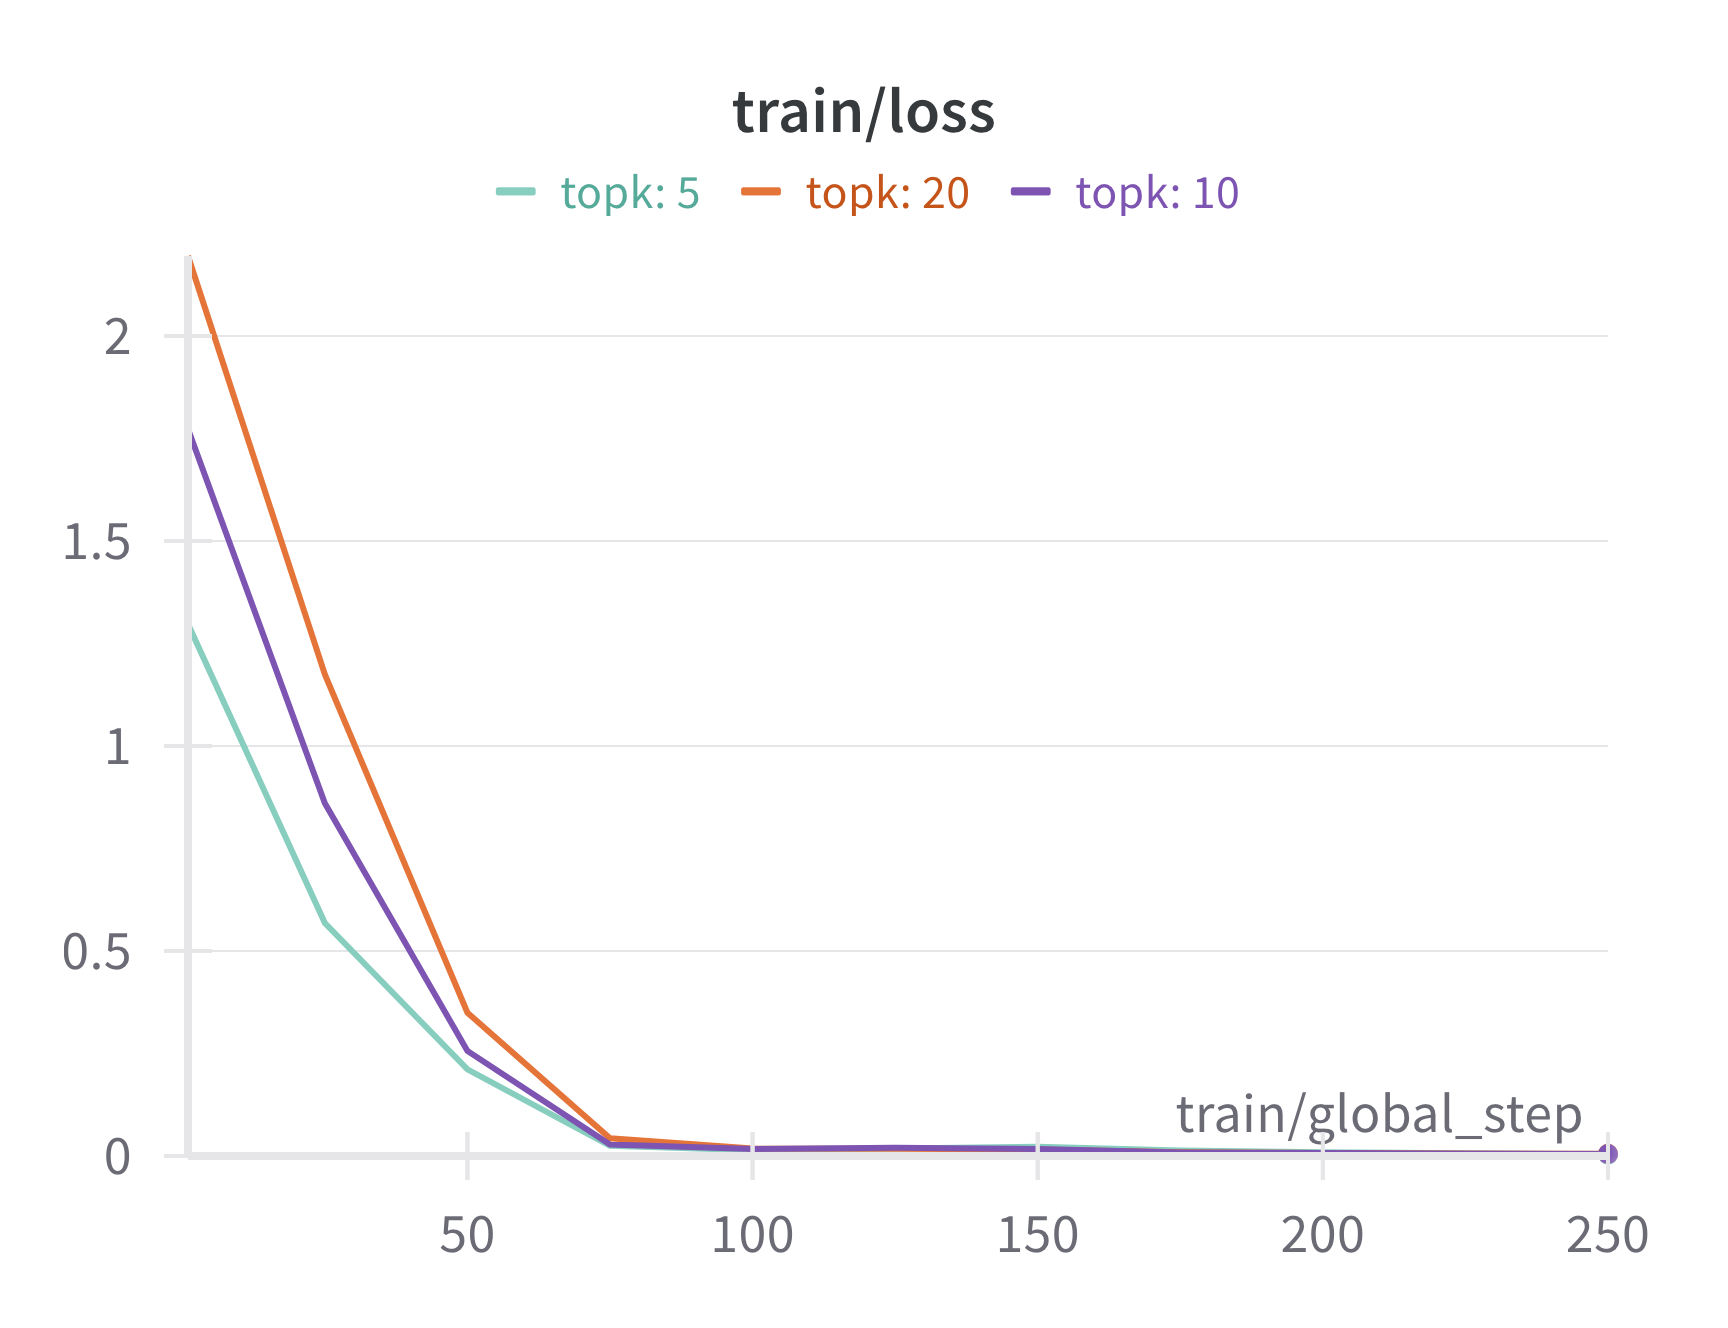
\includegraphics[width=0.50\textwidth]{Fig2_comparing topk.png}
   \caption{PBFT when different number of context examples provided}
   \label{fig:your-label}
\end{figure}



\begin{figure}[htbp]
   \centering
   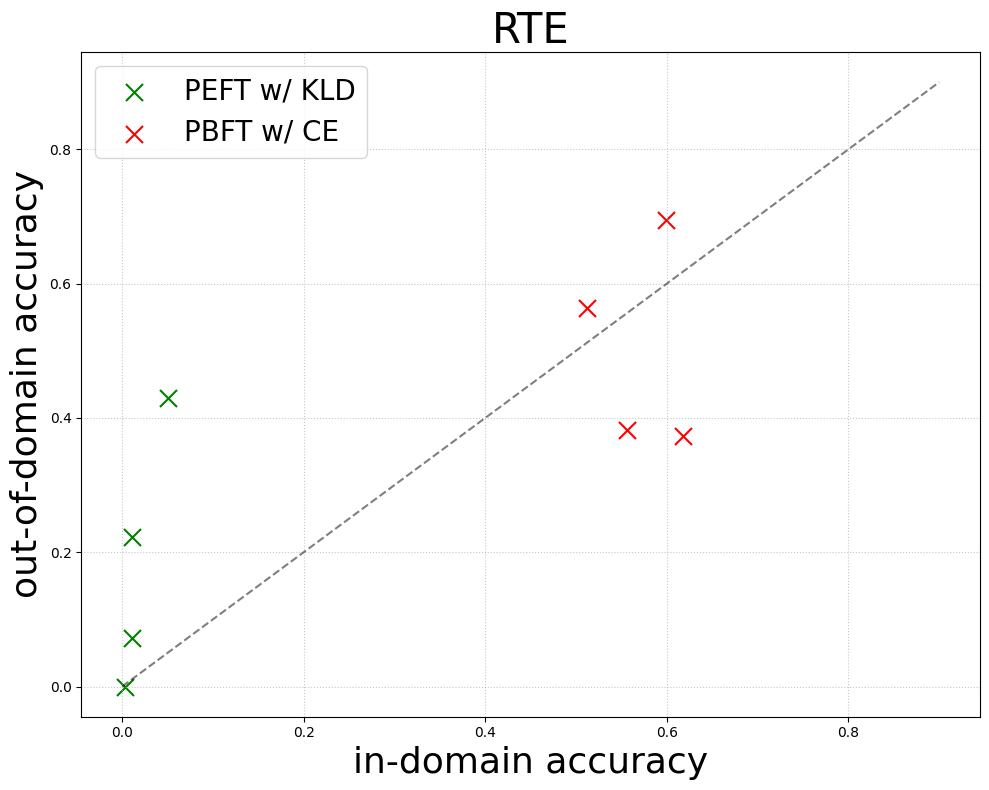
\includegraphics[width=0.50\textwidth]{Fig4_CE_KLD_comparing_id_ood.png}
   \caption{in-domain and out-of-domain accuracy between PBFT with DL divergence loss and CE loss}
   \label{fig:your-label}
\end{figure}


%-------------------------------------------------------------------------
\section{Discussion, conclusions, and future work}
\subsection*{Discussion}
The result showed the in-domain performance closer to 0 and some but definitely underperforming out-of-domain performance. We looked further into the predictions and it turns out the model did not limit its answers to only 0 or 1 the whole time. When we look further into the loss calculation, we realize the part predicting P0 was the issue. Thought the KL divergence loss helps approximating $P_\theta(X)$ to $P_0(X\mid C)$. The $_0(X\mid C)$ was not a meaningful prediction initially.
We investigated our experimentation setup and codes, and concluded several possibilities.
\subparagraph*{Small model size}
We’ve experimented with the opt model with 125 million parameters only due to limited resources. In the llmft paper, the experimentation was performed on much larger pre-trained models.
unbalanced examples 
We later realize that the examples we provide during fine tuning were not balanced. For example, when we supply 3 examples, the number of positive and negative examples can not be equal. and especially when we only supply 1 example, the pre-trained model was only shown 1 positive or negative example. 
KL divergence loss setup

In the experiments, we set up the KL divergence loss to select the top K tokens. After experiments, we realize the possibility that the expected outcome, 0 or 1, may not exist in the top K tokens initially. Taking it further, if we were never interested in tokens other than 0 or 1, it’s better and more straight-forward if we only select token 0 and 1 in the KL divergence loss setup.

\subparagraph*{Conclusions}
In summary, our experiments shows that  optimizing KL divergen loss with p0(X|C) is helpful, but due to the P0(X|C) part has some issues, we were not able to get some meaningful accuracy numbers that can be compared to the ICL approach.

\subparagraph*{Future work}
1. Experiment with larger model sizes: Use larger pre-trained models for P0 to potentially improve the quality of the context enriched predictions\\
2. Investigate hybrid loss functions: Experiment with combinations of KL divergence loss and cross-entropy loss.\\
3. Analyze context window size impact: Conduct experiments with varying context window sizes to determine the optimal length for different tasks and model sizes.




%-------------------------------------------------------------------------
\newpage
\newpage
\section{Work Division}

\begin{table*}
   \begin{center}
   \begin{tabular}{|c|p{4cm}|p{8cm}|}
   \hline
   Name & Contributed Aspects & Details \\
   \hline
   \hline
   Rilsky Viktor & Research. Design and implementation of the loss method. & Wrote the proposal and planned the scope of the project. Planned how we will implement the context distillation. Implemented the KLD loss. Initiating and flow of $P_0$ and $P_\theta$ models. Reading the original repo and planning where we should implement things and how. Coordinated with team members and organized tasks for everyone. \\
   \hline
   Pandurangan Suriyanarayna G & Implementation of the context prompting. Debugging. Supported the running of the experiments. &   Implemented the augmented dataset that draws enriches a sample with other samples as context. Helped for many long hours to pair-debugging many issues we encountered, both in implementation and experiments. Also added quality of life additions to the script so experiments are more organized. Suriyanarayna was involved in all parts of the code implementation and many things ran smoothly thanks to his efforts. \\
   \hline
   Lu Shuyan & Research, experiment design, experiment analysis.  & Did wide yet deep research and reading about the field and other solutions made to address the issue. Gave valuable perspectives on the scope and focus we should encompass. Designed the metrics and how we will evaluate our method. Examined the various solutions to the problem and compared how theoretically our proposition comes into play. Analyzed the experiment's results and concluded multiple points where we should have done things better. Lucy is a sharp scientist that led multiple discussions where she navigated and set the project goals. \\
   \hline
   Kim Hoyeob  & Implementation of the context prompting. Running the experiments. & Implemented the creation of the prompt $X \mid C$. Debugged many practical runtime issues and was successful in executing our scripts on remote cloud hardware. Collected the experiments in an organized manner. For hyperparameter tuning, ran the model dozens of times. Created graphs to visualize results. Prepared report formats and conducted reviews. Kim was a valuable member with high participation and was involved in coding, data analysis, visualization, and discussion of the results.

   \\
   \hline
   \end{tabular}
   \end{center}
   \caption{Contributions of team members.}
   \label{tab:contributions}
   \end{table*}


%------------------------------------------------------------------------

%-------------------------------------------------------------------------


{\small
\bibliographystyle{ieee_fullname}
\bibliography{egbib}
}

\end{document}
